\documentclass{article}

% Packages.

% Writing.
\usepackage[utf8]{inputenc}
\usepackage[english]{babel}
\usepackage{enumitem} % Enumerate using letters (\begin{description}[\alph]).

\usepackage{subfiles}

% Drawing, tables and images.
\usepackage{graphicx}
\usepackage{subfigure}
\usepackage{float} % Help in table and image positioning.
\usepackage{qtree}
\usepackage{tikz}
\usepackage{svg}

% Code.
\usepackage{minted}
\usemintedstyle{tango}
\definecolor{bg}{rgb}{0.95,0.95,0.95}


% Math.
\usepackage{mathtools} % Overbrackets.
\usepackage{amsmath} % Symbols.
\usepackage{amsthm} % Theorems.
\usepackage{amssymb} % Mathbb{}.
\usepackage{stmaryrd} % Brackets.
\usepackage{semantic}
\usepackage{relsize}
\usepackage{braket}

% Exercises.
\usepackage{exercise, chngcntr}
\counterwithin{Exercise}{section}
\counterwithin{Answer}{section}

% New commands.

% Theorems.
\newtheorem{Osservazione}{Osservazione}[section]
\newtheorem{Definition}{Definition}[section]
\newtheorem{Teorema}{Teorema}[section]
\newtheorem{Lemma}{Lemma}[section]
\newtheorem{Corollario}{Corollario}[section]
\newtheorem{thm}{Thm}[section]

\newcommand*{\uepsilon}{\underline{\epsilon}}
\newcommand*{\uempty}{\underline{\varnothing}}
\newcommand*{\ucdot}{\mathbin{\underline{\mathord{\cdot}}}}
\newcommand*{\lpar}{\underline{(}}
\newcommand*{\rpar}{\underline{)}}
\newcommand*{\ersem}[1]{\llbracket #1 \rrbracket}
\newcommand*{\bigersem}[1]{\bigl\llbracket #1 \bigr\rrbracket}
\newcommand*{\match}{\mathrel{\lessdot}}
\newcommand*{\nmatch}{\mathrel{\not\!\!\lessdot}}
\newcommand*{\Nset}{\mathbb{N}}
\newcommand*{\Rset}{\mathbb{R}}
\newcommand*{\defeq}{\mathrel{:=}}
\newcommand*{\sseq}{\subseteq}
\newcommand*{\ttt}{\texttt}
\newcommand*{\card}[1]{\lvert #1 \rvert}
\newcommand*{\powset}[1]{\wp(#1)}
\newcommand*{\powsetf}[1]{\wp_{f}(#1)}
\newcommand*{\st}{\mathrel{.}} % Such that, to be used with \exists.
\newcommand*{\itc}{\mathrel{:}} % It is the case that, to be used with \forall.
\newcommand*{\hd}{\hat{\delta}}
\newcommand*{\cd}{\check \delta}
\newcommand*{\ep}{\epsilon}
\newcommand*{\epstep}{\epsilon\text{-step}}
\newcommand*{\epclos}{\epsilon\text{-closure}}
\newcommand*{\rel}{\mathrel R}
\newcommand*{\nrel}{\mathrel{\not\!\!R}}
\newcommand*{\qt}{q_{\varnothing}}
\newcommand*{\ra}{\rightarrow}
\newcommand*{\grder}{\stackrel{G}{\Rightarrow}}
\newcommand*{\grderp}{\stackrel{G'}{\Rightarrow}}
\newcommand*{\grders}{\stackrel{G''}{\Rightarrow}}
\newcommand*{\grdef}{\mathrel{\mathord{:}\mathord{:}\mathord{=}}}
\newcommand*{\gralt}{\mathrel{\mid}}
\newcommand*{\defpar}{\rightarrowtail}
\newcommand*{\compl}[1]{\overline{#1}}
\newcommand*{\qmarrow}{\stackrel{\text{\larger{\textbf{?}}}}{\Longrightarrow}}
\newcommand*{\twodots}{\mathrel{. \, .}}


\def\checkmark{\tikz\fill[scale=0.4](0,.35) -- (.25,0) -- (1,.7) -- (.25,.15)
  -- cycle;}

\title
{
  Qudoku: solving Sudoku using Grover's algorithm \\
  \vspace*{1em}
  \large Quantum Computing\\
         Computer Science Master Degree\\
         University of Parma
}

\author{
  Federico Serafini\\
  \normalsize \texttt{federico.serafini@studenti.unipr.it}
}

\date{08/02/2023}

\begin{document}

\begin{titlepage}
  \clearpage\maketitle
  \thispagestyle{empty}
\end{titlepage}


\tableofcontents
\newpage

\section{Introduction}
Many interesting problems that computer science tries to solve are \emph{search
problems} over \emph{structured} and \emph{unstructured} databases.
The best algorithm for searching a winning element $\omega$ in a structured
database, a sorted list of $N$ elements for example, is the \emph{binary
search}: it allows to find $\omega$ in $\mathcal{O} (\log N)$ tries exploiting
data ordering.
Things get more difficult when the search is done over a list of $N$
randomly-placed elements.
Using a classical algorithm there is no way of taking advantage of
the data structure to speed up the search:
in the worst case, where the searched element is at the end of the list, a scan
over all the $N$ elements of the list is required.
In the average case, the number of tries to find $\omega$ is $N/2$.
So, the overall time complexity is $\mathcal{O}(N)$ and this means that time
cost for classical unstructured search algorithms grows linearly with the size
of the input.

In this report, we are going to discuss a new search
algorithm based on quantum computation: Grover's algorithm.
When searching any database (structured or unstructured), Grover's algorithm
time complexity is $\mathcal{O}(\sqrt N)$, which for unstructured
search is a quadratic improvement over the best classical algorithm.
It can serve as a general subroutine to
obtain quadratic run time improvements for a variety of other algorithms
through \emph{amplitude amplification trick}.
In particular, we are going to see a simple example of conversion from a
classical search problem as solving a binary Sudoku, into oracles for Grover's
algorithm.
\begin{figure}[H]
  \centering
  \includesvg[width=200pt]{Img/rg-vs-grover.svg}
  \caption{Time complexity.}
\end{figure}

\section{Basic concepts}

\subsection{Definitions}

\paragraph{Decision problem}
In computability theory and computational complexity theory, a
\emph{decision  problem} is a computational problem that can be posed as a
yes/no question of the input values.
A decision problem can be defined using two sets:
\begin{enumerate}
  \item
  $C$ as candidates, set all possible inputs;
  \item
  $W$ as winning elements, set of inputs for which the answer is yes.
\end{enumerate}
In our case, it will be useful to formulate the Sudoku as a decision problem,
where $C$ is the set composed by all $n^{n^2}$ different ways of filling a
$n \times n$ board, and $W$ set of valid solutions.

\paragraph{Oracle}
Many quantum algorithms are based around the analysis of some \emph{oracle}
function $f$: a ``black box" which we can give an input $x$
and receive the corresponding output $f(x)$.
Our objective is to determine some properties of the oracle function using the
minimum number of queries.

\subsection{Phase kickback}
\subsubsection{Rotations and eigenvalues}
If a gate $U$ rotates by the same amount all the amplitudes of a
state vector $\ket{x}$, then $\ket{x}$ is an eigenstate of that gate $U$ and,
as a result, $U$ acting on $\ket{x}$ will add a global phase $\theta$:
\[
  U \ket{x} = \lambda \ket{x} = e^{2 \pi i \theta} \ket{x}.
\]
For example, performing an $X$-gate on a $\ket{-}$ qubit gives it the phase
$-1$:
\begin{align*}
  X \ket{-}
  & = \tfrac{1}{\sqrt{2}}  \bigl( \ket{0}\bra{1} + \ket{1}\bra{0} \bigr)
      \bigl( \ket{0} - \ket{1} \bigr) \\
  & = \tfrac{1}{\sqrt{2}} \bigl( \ket{0}\bra{1} + \ket{1}\bra{0} \bigr)
      \bigl( \ket{0} - \ket{1} \bigr) \\
  & = \tfrac{1}{\sqrt{2}} \bigl( \ket{0}\braket{1|0} - \ket{0}\braket{1|1}
     + \ket{1}\braket{0|0} - \ket{1}\braket{0|1}  \bigr) \\
  & = \tfrac{1}{\sqrt{2}} \bigl( -\ket{0}  + \ket{1} \bigr) \\
  & =  - \tfrac{1}{\sqrt{2}} \bigl( \ket{0}  - \ket{1} \bigr) \\
  & =  - \ket{-}.
\end{align*}

\subsubsection{Kick back}
\emph{Phase kickback} is where the eigenvalue added by a gate to a qubit is
``kicked back" into a different qubit via a controlled operation.
When the control qubit is in either $\ket{0}$ or $\ket{1}$, this phase affects
the whole state, however it is a global phase and has no observable effects:
\begin{align*}
  CX \ket{-0}
  & = \ket{-} \otimes \ket{0} \\
  & = \ket{-0},
\end{align*}
\begin{align*}
  CX \ket{-1}
  & = X\ket{-} \otimes \ket{1} \\
  & = -\ket{-1} \\
  & = \ket{-1}.
\end{align*}
Things get interesting when the control qubit is in a superposition of
$\ket{0}$ and $\ket{1}$.
The component of the control qubit that lies in the direction of  $\ket{1}$
applies this phase factor to the corresponding target qubit and this applied
phase factor introduces a relative phase back to the control qubit:
\[
CU \ket{x} \bigl(\alpha \ket{0} + \beta \ket{1} \bigr) =
\ket{x} \bigl(\alpha \ket{0} + \beta e^{2 i \pi \theta} \ket{1} \bigr).
\]
For example:
\begin{align*}
  CX \ket{-+}
  & = \tfrac{1}{\sqrt{2}} \bigl( \ket{-0} + X\ket{-1} \bigr) \\
  & = \tfrac{1}{\sqrt{2}} \bigl( \ket{-0} - \ket{-1} \bigr) \\
  & = \ket{-} \otimes \tfrac{1}{\sqrt{2}} \bigl( \ket{0} - \ket{1} \bigr) =
      \ket{--}.\\
\end{align*}
This interesting quantum effect is a building block in many
famous quantum algorithms, including Grover's search algorithm.

\subsection{Oracles}

\paragraph{Classical oracle}
On classical algorithms, oracles can be seen as general functions:
\[
  f: \{\, 0, 1 \,\}^n \mapsto \{\, 0, 1 \,\}^m,
\]
where $n, m \in \Nset$ are the input and output length.

\paragraph{Boolean oracle}
In quantum computation, one of the main forms that oracles take is that of
\emph{boolean oracles}, described by the following unitary evolution:
\[
  U_f \bigl( \ket{x} \otimes \ket{y} \bigr) =  \ket{f(x) \oplus y},
\]
where:
\begin{itemize}
  \item
  $x$ is the input register ($n$ qubits, $n \geq 1$);
  \item
  $y$ is the output register ($m$ qubits, typically $m = 1$);
  \item
  $\oplus$ is an exclusive or.
\end{itemize}
Note that the result of applying $U_f$ depends on:
\begin{enumerate}
  \item
  $U_f$ definition;
  \item
  initial contents of both input and output registers, in particular,
  if $\ket{y} = \ket{0^m}$ then $\ket{f(x) \oplus y} = \ket{f(x)}$.
\end{enumerate}
\begin{figure}[H]
  \centering
  \includesvg{Img/grover-boolean-oracle.svg}
  \caption{Boolean oracle.}
\end{figure}

\paragraph{Phase oracle}
Another form of oracle used in quantum computation is the \emph{phase oracle},
defined as:
\[
  P_f \ket{x} = (-1)^{f(x)} \ket{x}.
\]
A phase oracle can be realized using boolean oracle and the phase kickback
mechanism (setting $\ket{y}$ in the state $\ket{-}$):
\[
  U_f \bigl( \ket{x} \otimes \ket{y} \bigr)
  = U_f \bigl( \ket{x} \otimes \ket{-} \bigr)
  = \bigl( P_f \otimes  I \bigr) \bigl( \ket{x} \otimes \ket{-} \bigr)
  = P_f \ket{x} \otimes \ket{-}
  = P_f \ket{x}.
\]
Input $x$ controls an $X$ rotation targeting the output qubit $y$ in state
$\ket{-}$:
if $f(x) = 1$ an $X$ rotation is applied to $\ket{-}$ resulting in a kickback
of the phase $-1$ on the state $\ket{x}$.
Qubit $y$ (whose state is left unchanged by the whole
process and can safely be ignored) it is called \emph{ancilla} qubit.
\begin{figure}[H]
  \centering
  \includesvg{Img/grover-phase-oracle.svg}
  \caption{Phase oracle.}
\end{figure}

\section{Grover's algorithm}

Now we are going to see how the Grover's algorithm works when searching for a
winning item $\omega$ among $N$ items.
Before diving into the details it can
be useful to visualize the shape of the circuit that implements it:
\begin{figure}[H]
  \centering
  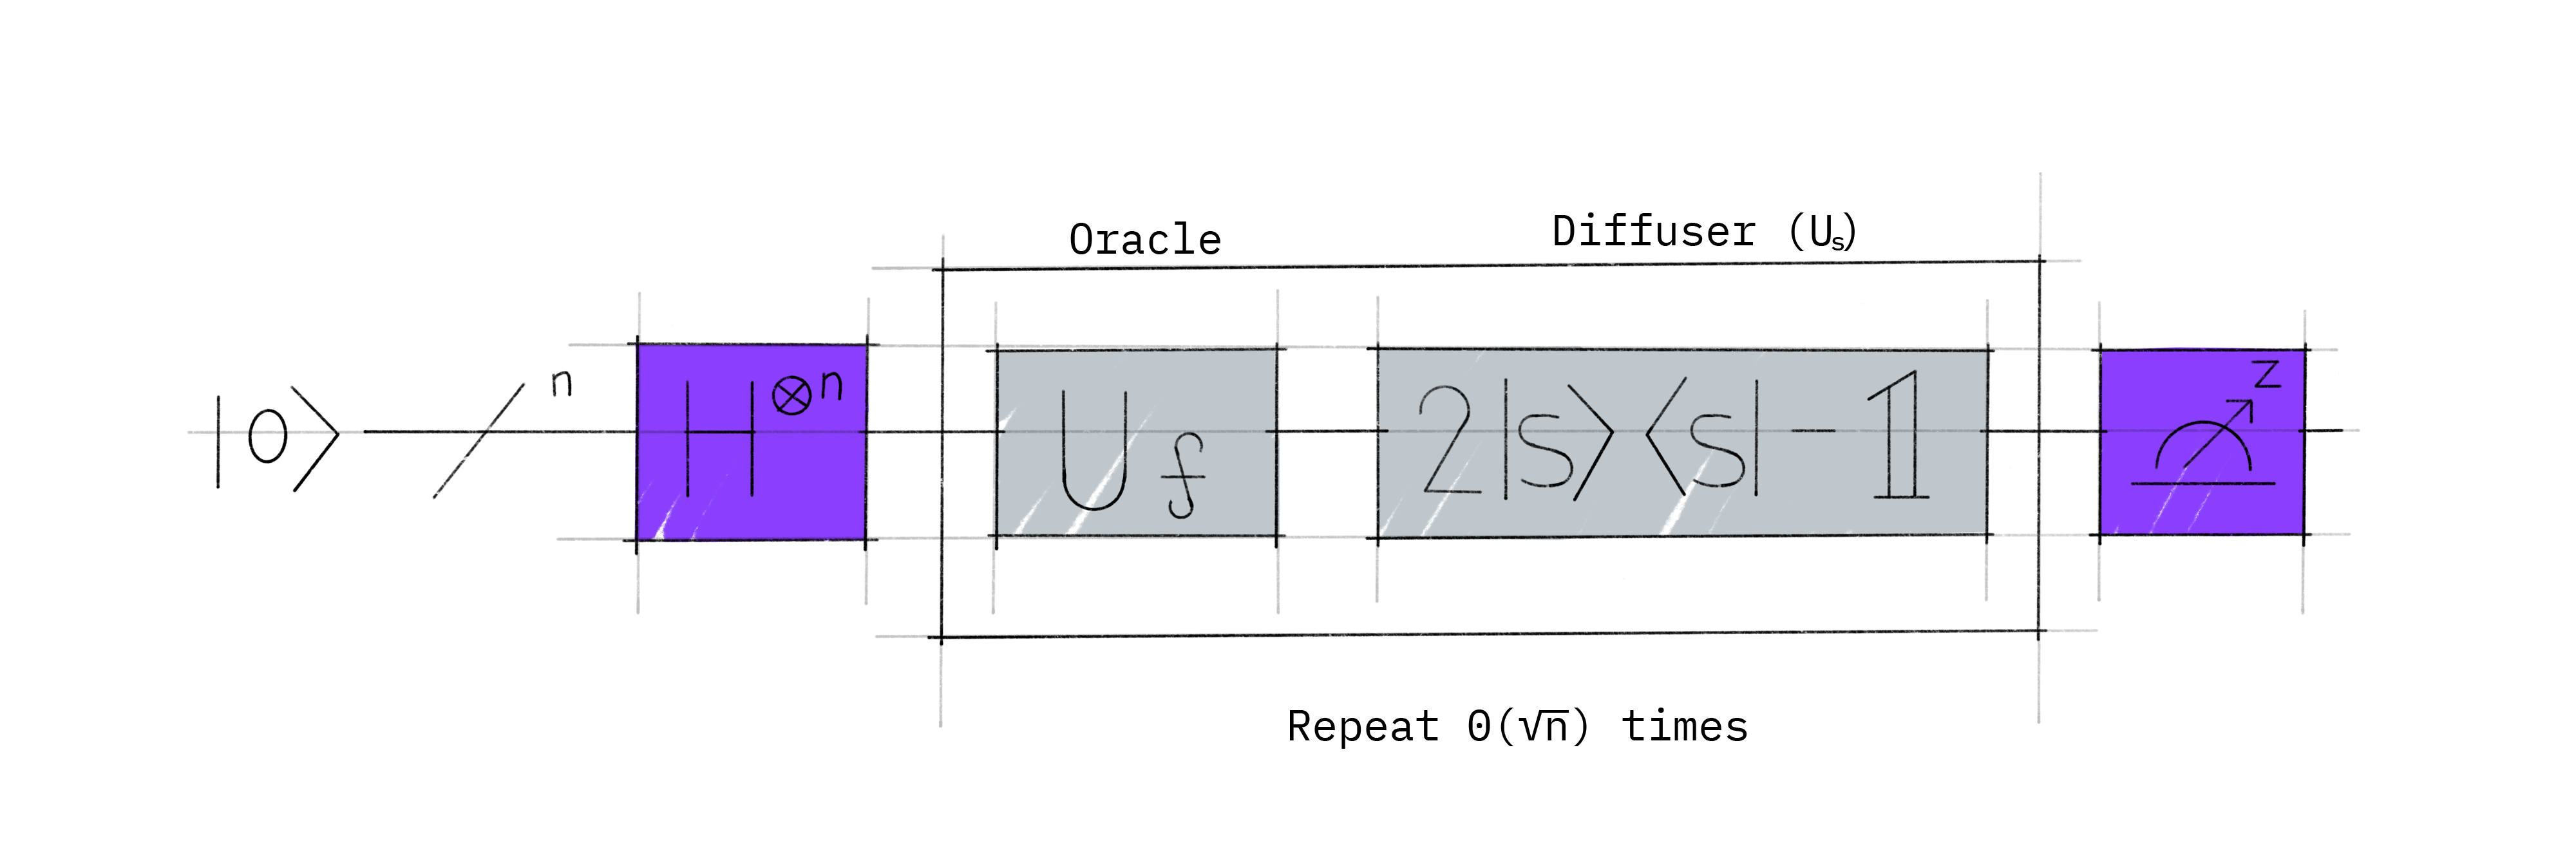
\includegraphics[width=345pt]{Img/grover-circuit-high-level.png}
  \caption{Grover's circuit.}
\end{figure}

\subsection{Preparation}
Before looking at the list of items, we have no idea where the winning item
is. Therefore, any guess of its location is as good as any other, which can be
expressed in a equal superposition of
  every possible input:
  \[
    H^{\otimes n} \ket{x} = \ket{s} = \frac{1}{\sqrt{2^n}} \sum_{k \in
    \{0, 1\}^n}
    \ket{k}
  \]
  We can create this superposition by applying a $H$-gate to each input qubit.

\subsection{Grover oracle}
Grover's oracle $U_\omega$ it is a phase oracle, so its application on an input
state $\ket{x}$ can be described as:
\[
  U_\omega \ket{x} = (-1)^{f(x)} \ket{x}.
\]
First thing we need to define is the \emph{indicator function} $f$.
A strong point of this algorithm is that it is \emph{general}:
definition of $f$ can vary depending on the search problem we are addressing.
In our case, the indicator function $f$ is defined as:
\[
  f(x) = \bigg\{
  \begin{aligned}
    1, && \text{if} \; x = \omega; \\
    0, && \text{otherwise}.
  \end{aligned}
\]
In general, there are many computational problems in which it’s difficult to
find a solution, but relatively easy to verify a solution; let $W$ be the
set of all valid solutions of a problem, then $f$ will be the function that
tell us if a candidate solution $x$ it is a valid solution or not.
\[
  f(x) = \bigg\{
  \begin{aligned}
    1, && \text{if} \; x \in W; \\
    0, && \text{otherwise}.
  \end{aligned}
\]
Given $f$, we can observe that Grove's oracle $U_\omega$ adds a negative
phase only to the winning element:
\[
  U_\omega \ket{x} = \bigg\{
  \begin{aligned}
    - \ket{x}, && \text{if} \; x = \omega; \\
    \ket{x},   && \text{otherwise}.
  \end{aligned}
\]
Another way of representing $U_\omega$ is taking an identity matrix $I$ and
adding a $-1$ phase to the winning element:
\[
  U_\omega =
  \begin{bmatrix}
    (-1)^{f(0)} &   0         & \cdots &   0         \\
    0           & (-1)^{f(1)} & \cdots &   0         \\
    \vdots      &   0         & \ddots & \vdots      \\
    0           &   0         & \cdots & (-1)^{f(2^n-1)} \\
  \end{bmatrix}
\]

\subsection{Amplitude amplification}
Finally it is time to apply the \emph{amplitude amplification} trick.
A procedure that amplifies the amplitude of the winning element,
which shrinks the other items' amplitude, so that measuring the final state
will return the right item with high probability.
Geometrically it corresponds of two reflections, which generate a rotation in a
two-dimensional plane.

\paragraph{Step 1}
Consider the vectors corresponding to the winner $\ket{\omega}$ and the
uniform superposition $\ket{s}$, these two vectors span a two-dimensional plane.
They are not perpendicular because $\ket{\omega}$
occurs in $\ket{s}$ with amplitude $\frac{1}{\sqrt{2^n}}$.
Let's consider an additional vector $\ket{s'}$ with the following
properties:
\begin{itemize}
  \item
  it is perpendicular to $\ket{\omega}$;
  \item
  in lays on the span of $\ket{\omega}$ and $\ket{s}$.
\end{itemize}
\begin{figure}[H]
  \centering
  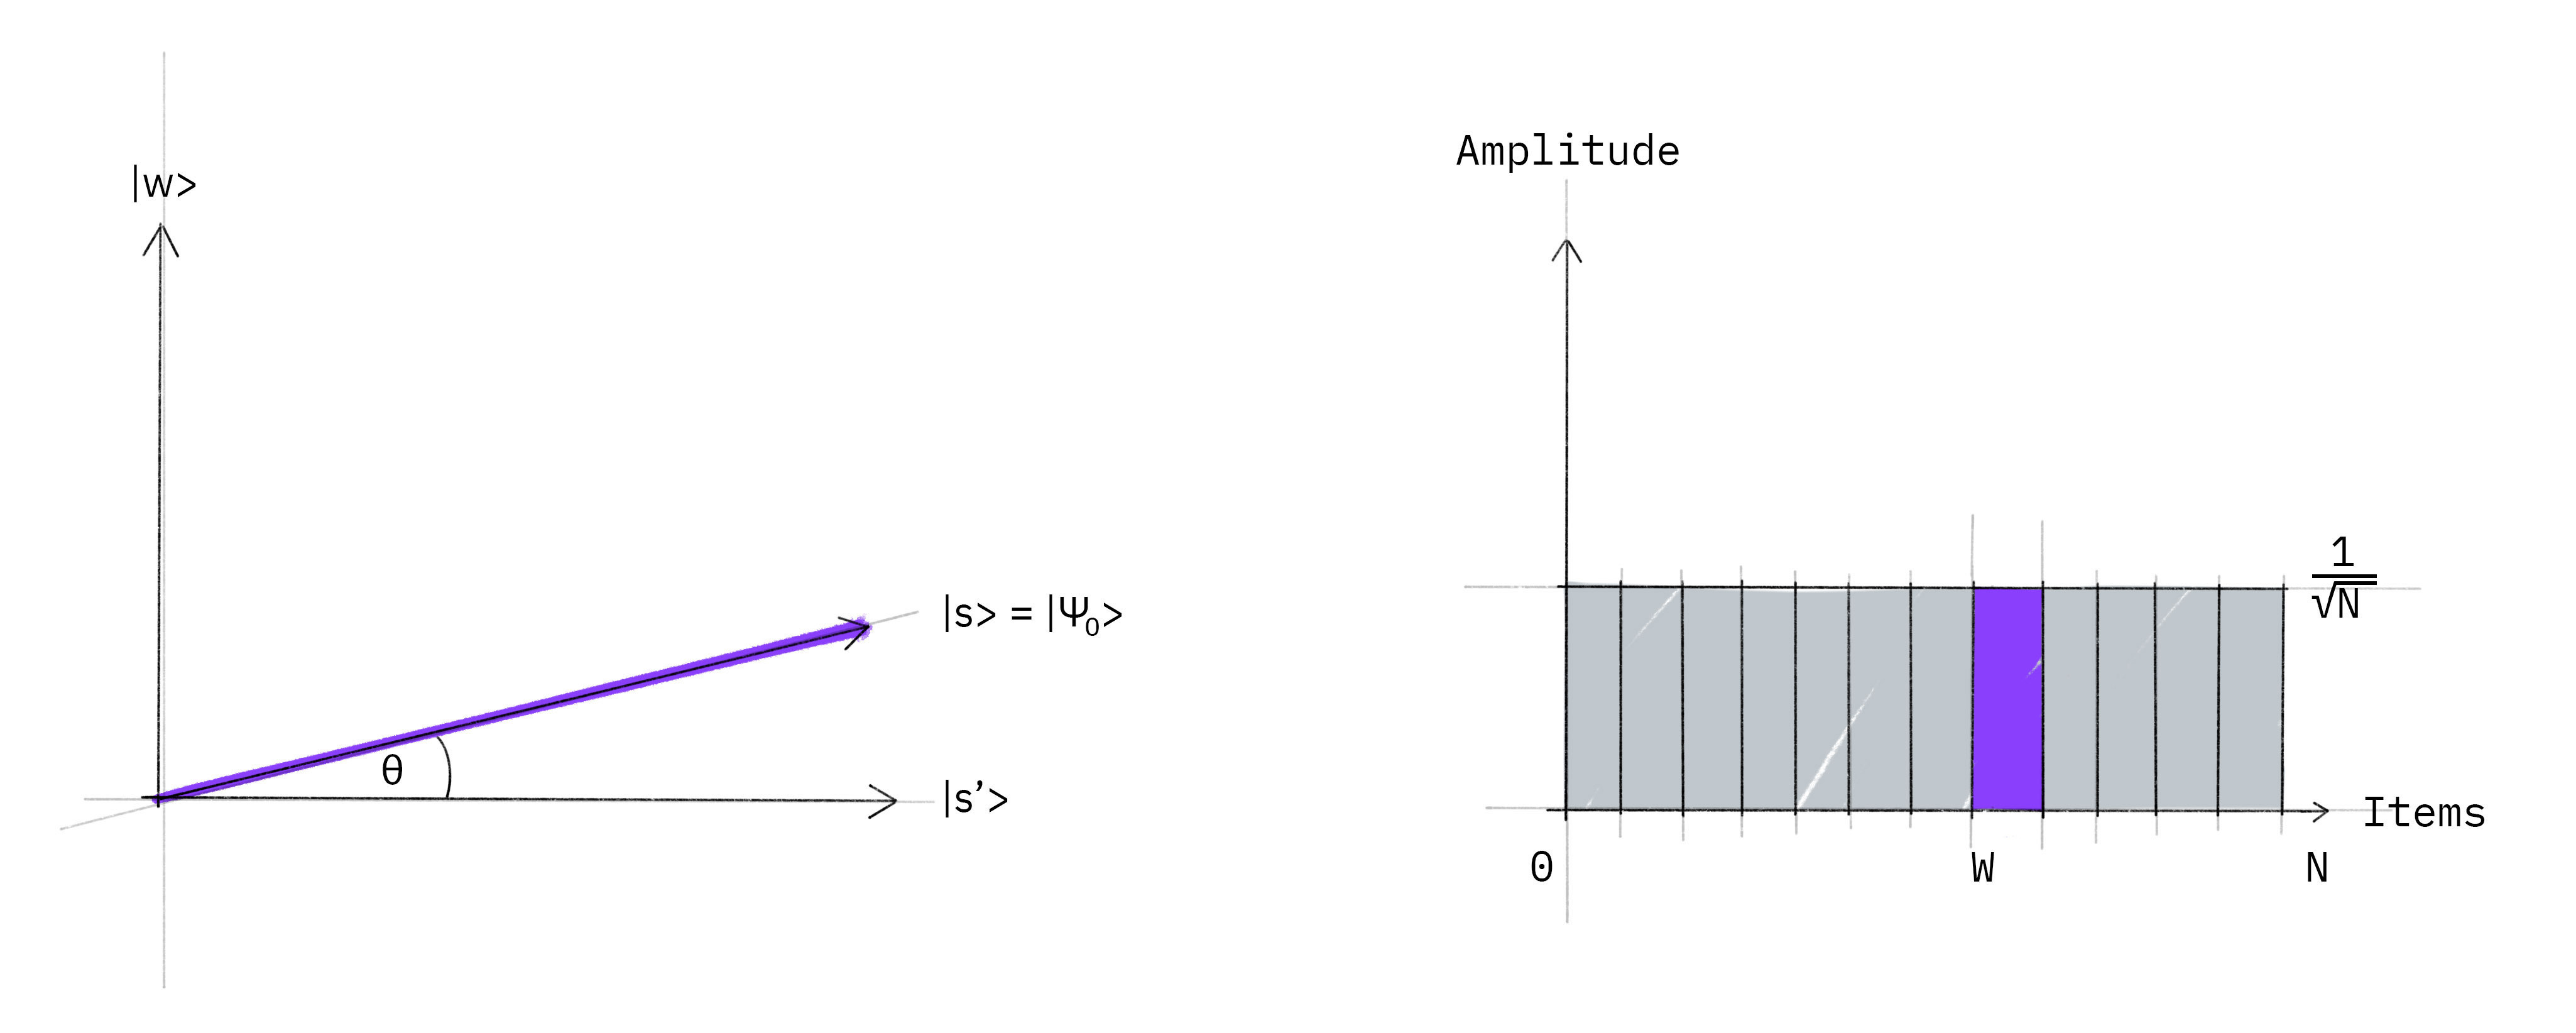
\includegraphics[width=300pt]{Img/grover-step1.jpg}
  \caption{$\ket{s} = H^{{\otimes}^n} \ket{x}$.}
\end{figure}

\begin{itemize}
  \item
  $\ket{s'}$ can be obtained from $\ket{s}$ by removing $\ket{\omega}$:
  $
    \ket{s'} = \tfrac{1}{\sqrt{2^n-1}} \sum_{k \neq \omega} \ket{k}.
  $
  \item
  $\ket{s}$ is a linear combination of $\ket{\omega}$ and $\ket{s'}$:
  \[
  \ket{s} = \tfrac{1}{\sqrt{2^n}}  \ket{\omega} + \sqrt{\tfrac{2^n-1}{2^n}}
  \ket{s'} = \sin{\theta} \ket{\omega} + \cos{\theta} \ket{s'},
  \]
  where $\sin{\theta} = \tfrac{1}{\sqrt{2^n}}$ is the
  amplitude af all the different states.
\end{itemize}

\paragraph{Step 2}
Now we apply the oracle $U_\omega$ to the superposition state
$\ket{s}$.
Geometrically, this corresponds to a reflection of the state $\ket{s}$
about $\ket{s'}$: the amplitude in front of the $\ket{\omega}$ becomes
negative, which in turn means that the average amplitude has been lowered.
\begin{figure}[H]
  \centering
  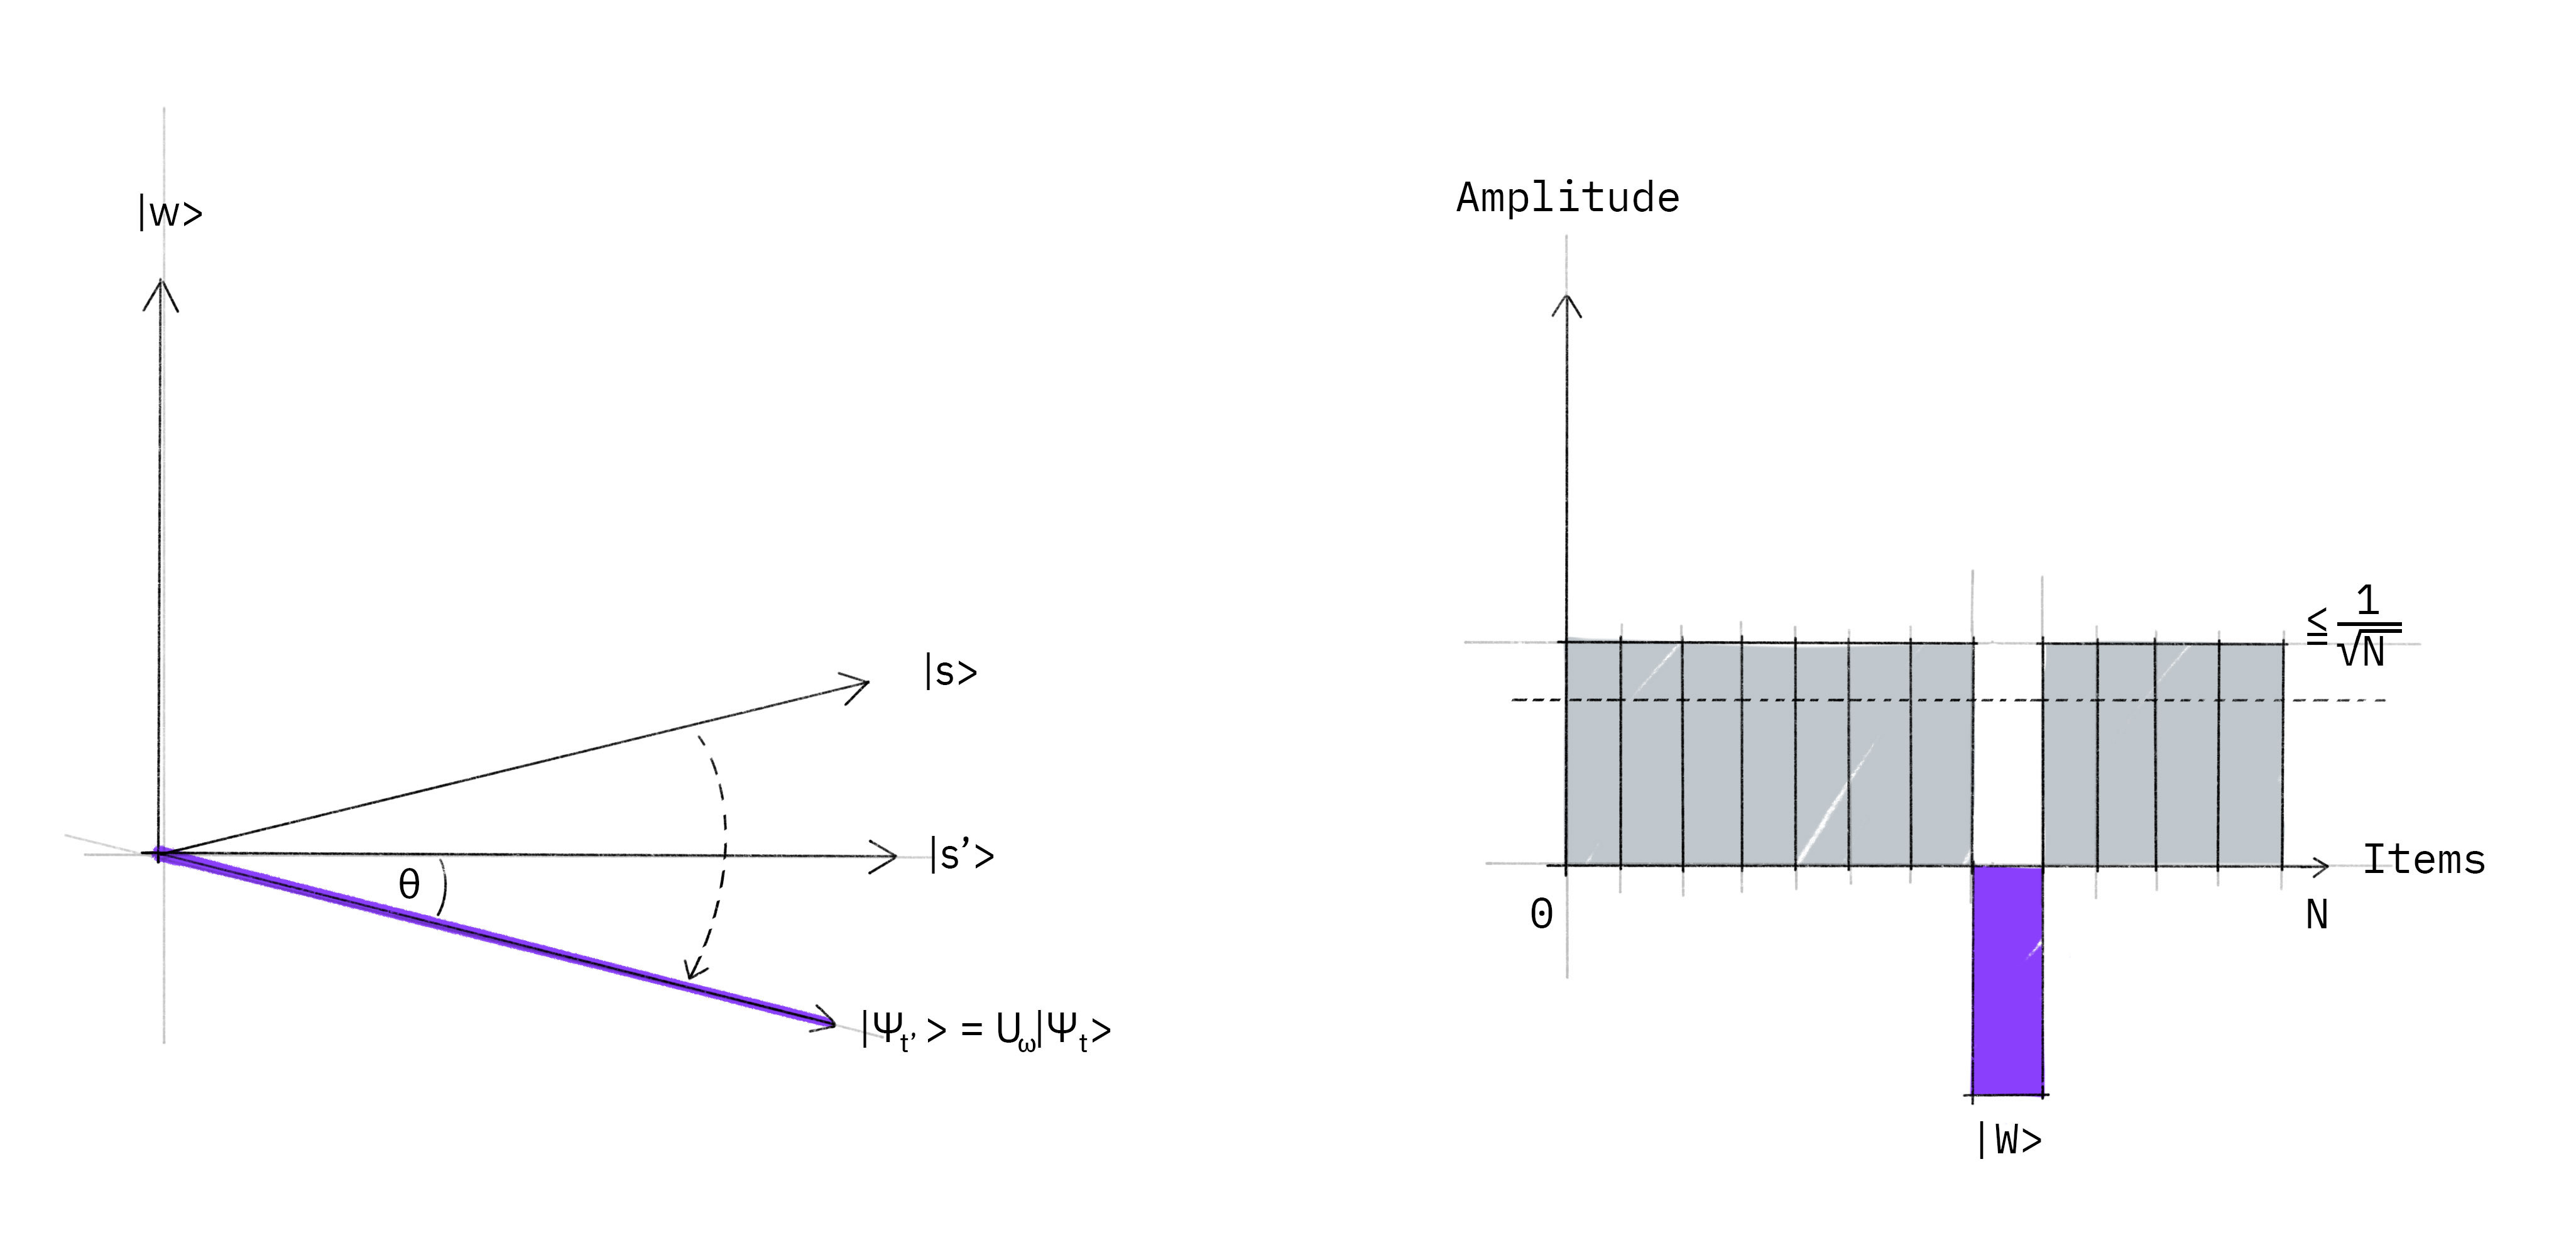
\includegraphics[width=300pt]{Img/grover-step2.jpg}
  \caption{$U_\omega \ket{s}$.}
\end{figure}

\paragraph{Step 3}
Apply the \emph{diffuser} $U_s = 2\ket{s}\bra{s} -I$ to the state $\ket{s}$.
Since this is a reflection about the state $\ket{s}$, we want to add a negative
phase to every state orthogonal to $\ket{s}$.
One way to do this is:
\begin{enumerate}
  \item
  transform $\ket{s} \rightarrow \ket{0^{\otimes n}}$ applying Hadamard gates;
  \item
  apply a negative phase to the states orthogonal to $\ket{0^{\otimes n}}$ using
  $
    U_0 = X^{\otimes n} (MCZ) X^{\otimes n};
  $
  \item
  transform $\ket{0^{\otimes n}} \rightarrow \ket{s}$ applying H-gate again.
\end{enumerate}
Putting all together: $U_s = H^{\otimes n} X^{\otimes n} (MCZ) X^{\otimes n}
H^{\otimes n} = H^{\otimes n} U_0 H^{\otimes n}$.
\begin{figure}[H]
  \centering
  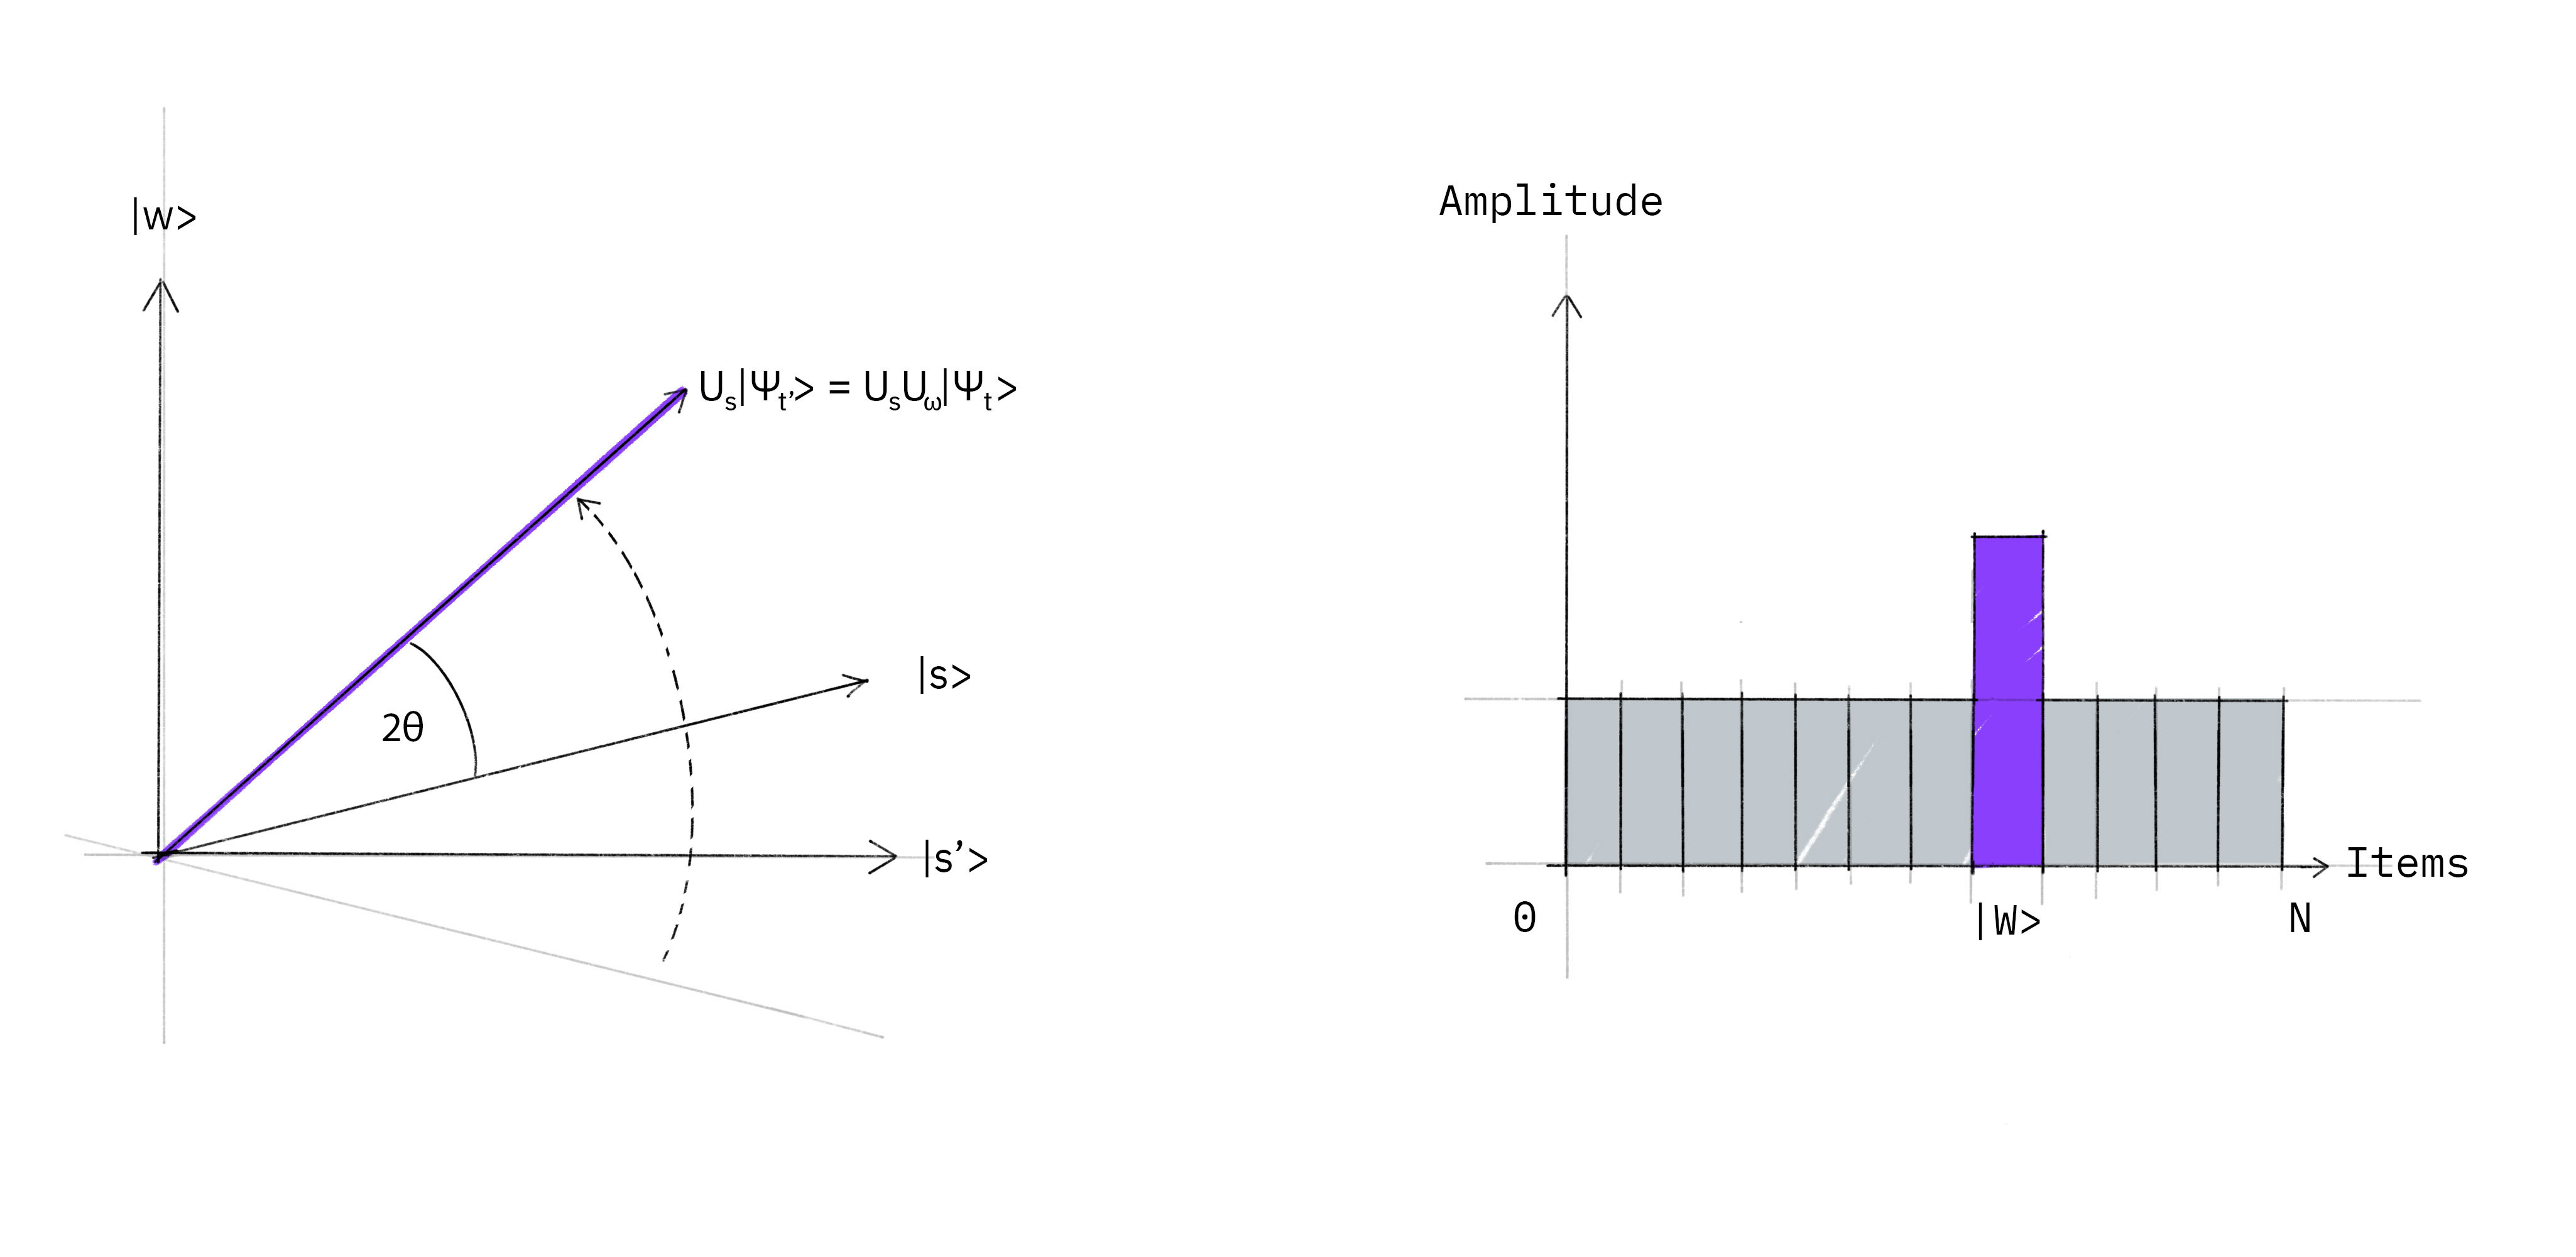
\includegraphics[width=300pt]{Img/grover-step3.jpg}
  \caption{$U_s U_\omega \ket{s}$}
\end{figure}
The transformation $U_s U_\omega \ket{s}$ rotates $\ket{s}$
closer towards the winner $\ket{\omega}$.
The action of the reflection
in the amplitude bar diagram can be understood as a reflection about the
average amplitude. Since the average amplitude has been lowered by the first
reflection, this transformation boosts the negative amplitude of
$\ket{\omega}$ to roughly three times its original value, while it decreases
the other amplitudes. We then go to step 2 to repeat the application.

\subsection{Repetitions}
\subsubsection{Single element}
Each application of steps 2 and 3, rotates $\ket{s}$
closer towards the winner $\ket{\omega}$ of an angle $2 \theta$.
We would like to find the minimum number of repetitions that brings us as close
as possible to $\ket{w}$: a $90^\circ$ rotation taking into account the initial
position of $\ket{S}$.
\begin{align*}
  & t(2 \theta) = \frac{\pi}{2} - \theta, \\
  & t = \frac{\pi}{4 \theta} - \frac{\theta}{2\theta}, \\
  & t = \frac{\pi}{4 \arcsin \bigl( {\sqrt{N} } \bigr) } - \frac{1}{2},\\
  & t = \frac{\pi}{4} \sqrt{N} - \frac{1}{2} =
  \mathcal O(\sqrt{N}).
\end{align*}

\subsubsection{Multiple elements}
Let $M$ be the number of winning (or marked) elements.
Then the winning state $\ket{\omega}$ is defined as:
\[
  \ket{\omega} = \frac{1}{\sqrt{M}} \sum_{i = 1}^{M} \ket{\omega_i}.
\]
Then:
  \[
    \ket{s'} =
    \frac{1}{\sqrt{N-M}} \sum_{k \notin \{ \omega_1 \ldots \omega_M \}} \ket{k},
  \]
  \[
    \ket{s} =
    \sqrt{\frac{M}{N}} \ket{\omega} + \sqrt{\frac{N-M}{N}} \ket{s'}
    = \sin\theta \ket{\omega} + \cos{\theta} \ket{s'}.
  \]
Angle $\theta$ becomes larger:
\[
  \theta = \arcsin \bigl( \sqrt{\frac{M}{N}} \bigr),
\]
and $t$ reduces:
\begin{align*}
  & t(2 \theta) = \frac{\pi}{2} - \theta, \\
  & t = \frac{\pi}{4 \theta} - \frac{\theta}{2\theta}, \\
  & t = \frac{\pi}{4 \arcsin \bigl( \sqrt{\frac{M}{N}} \bigr) } - \frac{1}{2},\\
  & t = \frac{\pi}{4} \sqrt{\frac{N}{M}} - \frac{1}{2}
    = \mathcal O\biggl(\sqrt{\frac{N}{M}}\biggr).
\end{align*}

\newpage
\section{Solving Sudoku}
We will apply the Grover's algorithm to solve a $2 \times 2$ binary Sudoku.
Considering all the possible ways of filling the board, the search space size
is $N = 2^{4}$, and a candidate solution $x = \ket{v_3, v_2,
  v_1, v_0}$ is a binary number in the interval $[0 \twodots N-1]$.
\begin{figure}[H]
  \centering
  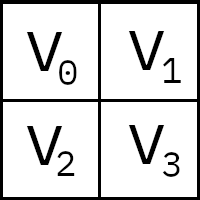
\includegraphics[width=50pt]{Img/binary-sudoku.png}
  \caption{Binary Sudoku.}
\end{figure}

\subsection{Circuit code}
\subsubsection{Global variables}
\begin{minted}[linenos, samepage, bgcolor=bg]{Python}
l = 2    # Borad length.
n = l*l  # Borad size.

# Row clauses: 0 != 1, 2 != 3.
# Col clauses: 0 != 2, 1 != 3.
clause_list = [[0, 1], [0, 2], [1, 3], [2, 3]]

# Registers.
var_qubits = QuantumRegister(n, name='v')     # Variables.
clause_qubits = QuantumRegister(n, name='c')  # Clause-checks.
out_qubit = QuantumRegister(1, name='out')    # f(x).
cbits = ClassicalRegister(n, name='cbits')    # Classical bits.
\end{minted}
\newpage
\subsubsection{Indicator function}
Let $W$ be the set of all valid
solutions (winning elements).
A candidate solution $x$ is considered valid ($x \in W$) if
the following conditions are met:
\begin{enumerate}
  \item
  no row may contain the same value twice ($v_0 \neq v_1, v_2 \neq v_3$);
  \item
  no columns may contain the same value twice ($v_0 \neq v_2, v_1 \neq v_3$).
\end{enumerate}
We can define our function $f$ as the indicator function of $W$:
\[
  f(x) = \bigg\{
  \begin{aligned}
    1, && \text{if} \; x \in W; \\
    0, && \text{otherwise}.
  \end{aligned}
\]

\begin{minted}[linenos, samepage, bgcolor=bg]{Python}
def f(n):

  qc = QuantumCircuit(var_qubits, clause_qubits)

  # Check every single clause using XOR.
  c = 0
  for clause in clause_list:
    qc.cx(clause[0], clause_qubits[c])
    qc.cx(clause[1], clause_qubits[c])
    c += 1

  # Return f as a gate.
  f = qc.to_gate()
  f.name = "f"
  return f
\end{minted}
\begin{figure}[H]
  \centering
  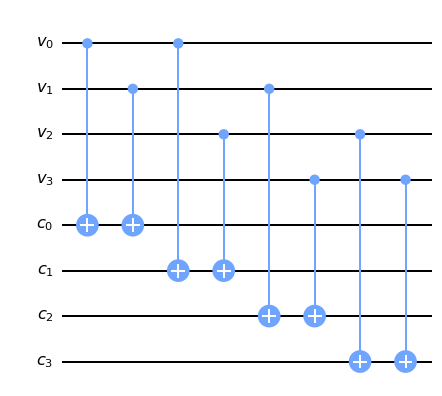
\includegraphics[width=210pt]{Img/f-circuit.png}
  \caption{Sudoku indicator function $f$.}
\end{figure}
\newpage
\subsubsection{Oracle}
\begin{minted}[linenos, samepage, bgcolor=bg]{Python}
def phase_oracle(n):

  qc = QuantumCircuit(var_qubits, clause_qubits, out_qubit)

  # Apply f.
  qc.append(f(n), range(2*n))

  # Flip out qubit if all clauses are satified.
  qc.mct(list(range(n, 2*n)), 2*n)

  # Apply f a second time to set clause qubits to |0>.
  qc.append(f(n), range(2*n))

  # Return oracle as a gate.
  U_f = qc.to_gate()
  U_f.name = "U_f"
  return U_f
\end{minted}
\begin{figure}[H]
  \centering
  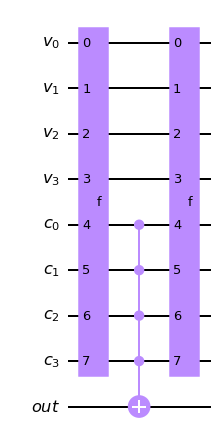
\includegraphics[width=130pt]{Img/uf-circuit.png}
  \caption{Sudoku oracle $U_f$.}
\end{figure}

\newpage
\subsubsection{Diffuser}
\begin{minted}[linenos, samepage, bgcolor=bg]{Python}
def diffuser(n):

  qc = QuantumCircuit(var_qubits)

  # Apply transformation |s> -> |00..0>.
  for qubit in range(n):
    qc.h(qubit)

  # Apply transformation |00..0> -> |11..1>.
  for qubit in range(n):
    qc.x(qubit)

  # Multi controlled Z-gate.
  qc.h(n-1)
  qc.mct(list(range(n-1)), n-1)
  qc.h(n-1)

  # Apply transformation |11..1> -> |00..0>.
  for qubit in range(n):
    qc.x(qubit)

  # Apply transformation |00..0> -> |s>.
  for qubit in range(n):
    qc.h(qubit)

  # Return the diffuser as a gate.
  U_s = qc.to_gate()
  U_s.name = "U_s"
  return U_s
\end{minted}
\begin{figure}[H]
  \centering
  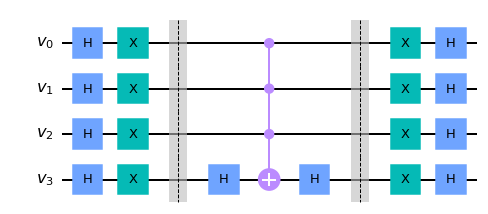
\includegraphics[width=300pt]{Img/us-circuit.png}
  \caption{Diffuser $U_s$.}
\end{figure}

\subsubsection{Amplitude amplification}
\begin{minted}[linenos, samepage, bgcolor=bg]{Python}
qc = QuantumCircuit(var_qubits, clause_qubits, out_qubit, cbits)

# Superposition.
for q in var_qubits:
  qc.h(q)

# Initialize 'out' in state |->.
qc.x(out_qubit)
qc.h(out_qubit)

# Amplification.
t = 2
for i in range(t):
  qc.append(phase_oracle(n), range(2*n +1))
  qc.append(diffuser(n), range(n))

# Measure the variable qubits.
qc.measure(var_qubits, cbits)
\end{minted}
\begin{figure}[H]
  \centering
  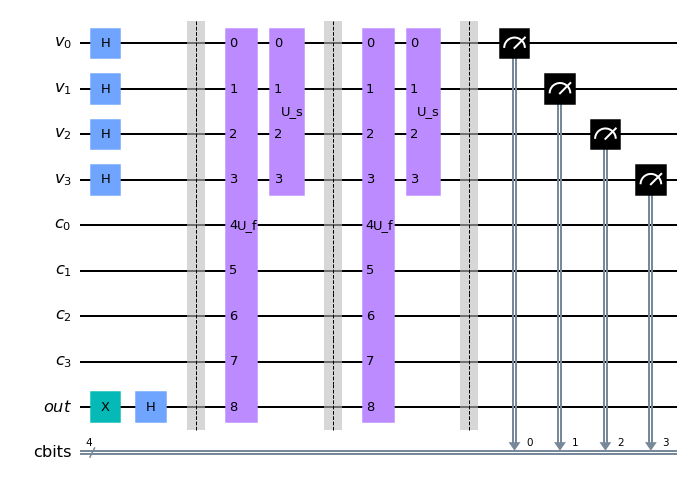
\includegraphics[width=320pt]{Img/circuit.png}
  \caption{Solving Sudoku circuit.}
\end{figure}

\subsection{Ideal simulation}
\begin{figure}[H]
  \centering
  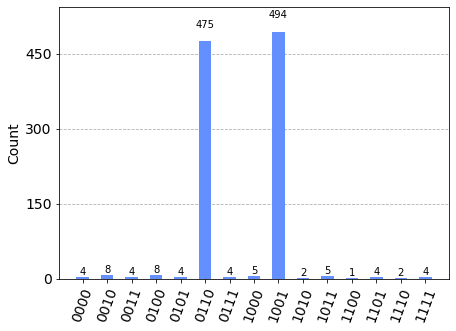
\includegraphics[width=250pt]{Img/simulation-t2.png}
  \caption{circuit simulation $t=2$.}
\end{figure}
From the results of $1024$ ideal simulations of our circuit we can observe that
the phase amplification trick it is working properly and it is really powerful.
In our case, following the theory and knowing in advance that $N = 2^4, M=2$,
we can find that:
\[
  t = \frac{\pi}{4} \sqrt{\frac{N}{M}}- \frac{1}{2} = \frac{\pi}{4}
  \sqrt{8}- \frac{1}{2} \approx 2.
\]
What happen with $t= 1$ or $t=3$? Result quality reduces:
\begin{figure}[H]
  \centering
  \begin{minipage}{.5\textwidth}
    \centering
    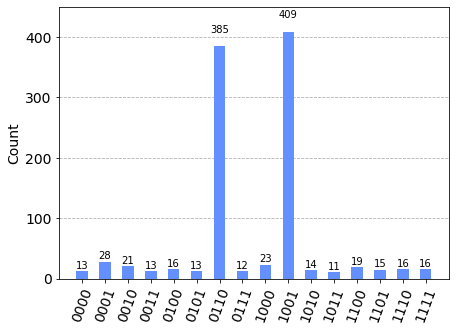
\includegraphics[width=6cm]{Img/simulation-t1.png}
    \caption{circuit simulation $t=1$.}
  \end{minipage}%
  \begin{minipage}{.5\textwidth}
    \centering
    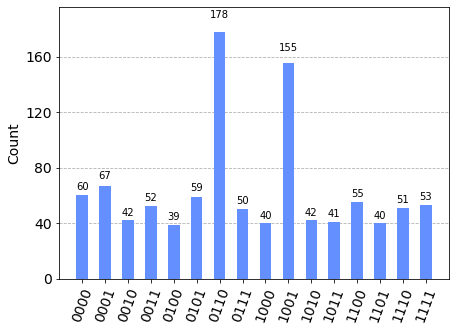
\includegraphics[width=6cm]{Img/simulation-t3.png}
    \caption{circuit simulation $t=3$.}
  \end{minipage}
\end{figure}

\section{Quantum error}
Theory seen so far assumes qubits can be prepared in any desired state and then
be manipulated with complete precision.
Qubits that obey these assumptions are often known as \emph{logical qubits},
but in reality, we are dealing with \emph{phisical qubits}: physical systems
that behave as qubits with some imperfections that lead to noisy results.

\subsection{Gate error: 1 and 2 qubits}
Determine effect of noise that occurs through a real quantum
computation is in general a complex problem:
each gate can introduce some noise and considering how each gate
transforms the effect of each error is not trivial.
These are the results after applying
$X$-gate error and $CX$-gate both at $p = 1\%$:
\begin{figure}[H]
  \centering
  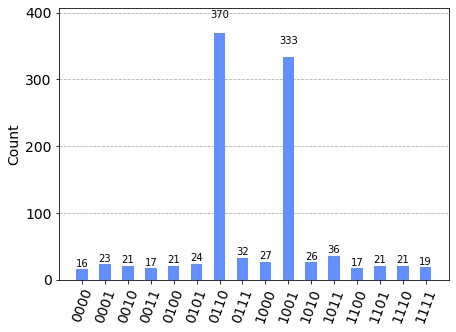
\includegraphics[width=250pt]{Img/error-g.png}
  \caption{$X$ and $CX$ errors $p = 1\%$.}
\end{figure}

\subsection{Thermal relaxation}
An even more realistic error model is based on \emph{thermal relaxation} with
the qubit environment:
\begin{itemize}
  \item
  each qubit is parameterized by a thermal relaxation time constant $T_1$
  and a dephasing time constant $T_2$;
  \item
  $T_2 \leq 2T_1$;
  \item
 error rates on instructions are determined by gate times and qubit $T_1, T_2$
 values.
\end{itemize}
\begin{figure}[H]
  \centering
  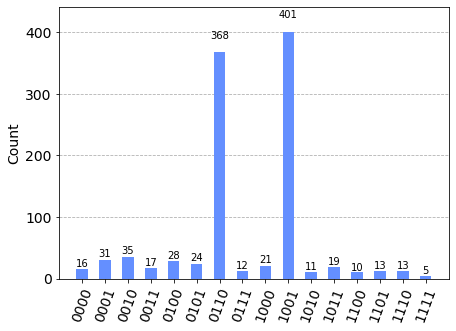
\includegraphics[width=250pt]{Img/error-r.png}
  \caption{thermal relaxation error.}
\end{figure}

\subsection{Measurement error and mitigation}
Let's now consider \emph{measurement error}, a simple form of noise occurring
during final measurements: each qubit is randomly perturbed with a probability
$p$.
\begin{figure}[H]
  \centering
  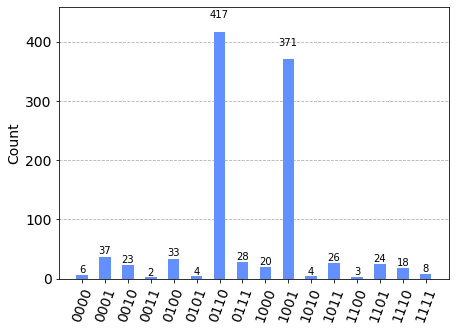
\includegraphics[width=250pt]{Img/error-m.png}
  \caption{measurement error $p = 5\%$.}
\end{figure}
It is possible to determine exactly what the effects of measurement errors
are preparing each of the possible basis states, measuring them, and
seeing what probability exists for each outcome.
Given $n$ qubits, following this procedure we are able to build a $2^n \times
2^n$ \emph{calibration matrix} $M$, where in position $i, j$ we can find the
probability of
measuring $\ket{i} = C_\text{noisy}$, given a qubit in the state
$\ket{j} = C_\text{ideal}$.
This is a good way of predicting noisy results given a knowledge of what the
results should be:
\[
C_\text{noisy} = M C_\text{ideal}.
\]
\emph{Measure error mitigation} is the process of computing $M$ and its
inverse $M^{-1}$ in order to find the ideal result:
\[
C_\text{ideal} = M^{-1} C_\text{noisy}.
\]
\begin{figure}[H]
  \centering
  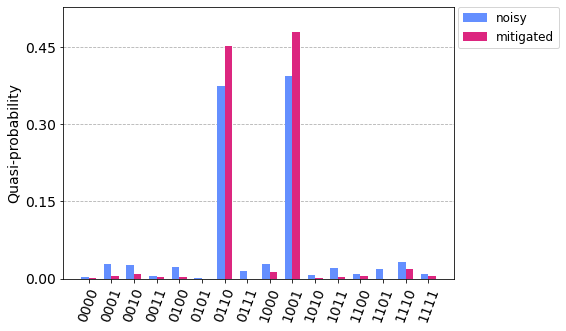
\includegraphics[width=335pt]{Img/error-m-mitigation.png}
  \caption{measure error mitigation $p = 5\%$.}
\end{figure}

In the current (NISQ: noisy intermediate-scale quantum) era,
physical qubits are used despite their imperfections:
a logical qubit can be encoded in a large number of physical qubits in
high-entangled circuits and using techniques as quantum error detection and
correction.

\section{Conclusion}
In this report, we explored all the basic concepts needed to understand
the Grover's algorithm: a search algorithm over an unstructured dataset that
gives a quadratic improvement over the best classical algorithm.
In particular we saw a conversion of classical decision problem
(solving Sudoku) into an oracle for Grover's algorithm, showing the ability to
solve problems for which we do not necessarily know the solution beforehand.

As future work, it would be interesting to inspect algorithm properties
when the problems size grows, paying particular attention to:
\begin{itemize}
  \item
  number of qubits needed to solve an $n \times n$ Sudoku, with $n \in \Nset$;
  \item
  noise impact;
  \item
  number of qubits needed for error detection and correction;
  \item
  when the number of solution $M$ is not known in advance, how can we
  compute the number of repetitions $t$?
\end{itemize}
\end{document}
